\documentclass[10pt,aspectratio=169]{beamer}
\usepackage[utf8]{inputenc}
\usepackage{listings}
\usepackage{hyperref}
\usepackage{xcolor}
\usepackage{ragged2e}
\usepackage{graphicx}
\usepackage{tikz}
\usetikzlibrary{positioning,calc,decorations.pathreplacing}

\usetheme{Dresden}
%\usetheme{Bergen}

\title{Programming Techniques 2026--2027}
\author{Hannu Parviainen}
\institute{Universidad de la Laguna}
\date{\today}

\lstset{
  language=fortran,
  basicstyle=\ttfamily\scriptsize,
  columns=fullflexible,
  keepspaces=true,
  backgroundcolor=\color{white},
  keywordstyle=\color{blue},
  commentstyle=\color{gray},
  stringstyle=\color{red},
  showstringspaces=false,
  breaklines=true,
  frame=lines
}

\subtitle{Lecture 12: Introduction to MPI}

\begin{document}

\begin{frame}
  \titlepage
\end{frame}


\section{Introduction}

\begin{frame}
  \frametitle{From OpenMP to MPI}
  \begin{columns}[T]
    \begin{column}{0.5\textwidth}
      \begin{itemize}
        \item \textbf{OpenMP} (Lectures 9 and 10): the threads of one program share the memory of one computer.
        \item \textbf{MPI}: many copies of the program run as separate \emph{processes}. Each process has its own memory, with its own copy of every variable.
        \item A process cannot see the variables of another one. The processes exchange data only by sending and receiving \emph{messages}.
        \item The processes can run on one computer, or on many nodes of a cluster.
      \end{itemize}
    \end{column}

    \begin{column}{0.5\textwidth}
      \centering
      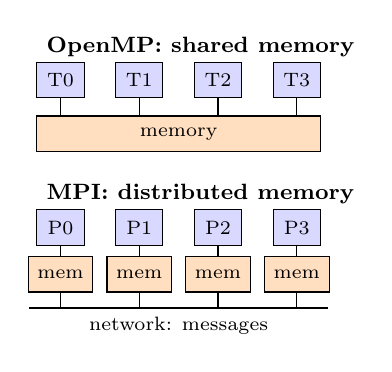
\begin{tikzpicture}[font=\scriptsize, y=0.85cm,
          cpu/.style={draw, fill=blue!15, minimum width=0.6cm, minimum height=0.45cm},
          mem/.style={draw, fill=orange!25, minimum height=0.45cm}]
        % Shared memory
        \node[anchor=west, font=\footnotesize\bfseries] at (-0.3,3.7) {OpenMP: shared memory};
        \node[mem, minimum width=3.6cm] (m) at (1.5,2.4) {memory};
        \foreach \i in {0,1,2,3} {
          \node[cpu] (t\i) at (\i*1.0,3.2) {T\i};
          \draw (t\i) -- (t\i |- m.north);
        }
        % Distributed memory
        \node[anchor=west, font=\footnotesize\bfseries] at (-0.3,1.5) {MPI: distributed memory};
        \foreach \i in {0,1,2,3} {
          \node[cpu] (p\i) at (\i*1.0,1.0) {P\i};
          \node[mem, minimum width=0.8cm] (m\i) at (\i*1.0,0.3) {mem};
          \draw (p\i) -- (m\i);
          \draw (m\i.south) -- (\i*1.0,-0.2);
        }
        \draw[thick] (-0.4,-0.2) -- (3.4,-0.2);
        \node[below] at (1.5,-0.2) {network: messages};
      \end{tikzpicture}

      \vspace*{1mm}
      \footnotesize
      \begin{tabular}{lll}
        & \textbf{OpenMP} & \textbf{MPI} \\
        \hline
        runs as & threads   & processes \\
        memory  & shared    & distributed \\
        scale   & one node  & many nodes \\
        \hline
      \end{tabular}
    \end{column}
  \end{columns}
\end{frame}


\begin{frame}
  \frametitle{What is MPI?}
  \begin{columns}[T]
    \begin{column}{0.5\textwidth}
      \begin{itemize}
        \item The \emph{Message Passing Interface} is a standard for a library of message-passing routines, with bindings for Fortran and C. The first version, MPI-1, was published in 1994, and the current one is MPI-5.0 (2025).
        \item The standard is implemented by several libraries: \textbf{Open MPI} and \textbf{MPICH} are free, and vendors such as Intel and HPE ship their own. A correct program works with all of them.
        \item MPI is the standard way to run programs on supercomputers.
      \end{itemize}
    \end{column}

    \begin{column}{0.5\textwidth}
      \begin{itemize}
        \item Usually every process runs the same program, and works on its own part of the data. This is called SPMD: \emph{single program, multiple data}.
        \item The processes are grouped into \emph{communicators}. \texttt{MPI\_COMM\_WORLD} contains all the processes.
        \item In a communicator of $p$ processes, each process has a number, its \emph{rank}, from 0 to $p - 1$. The program uses the rank to decide what each process does.
      \end{itemize}
    \end{column}
  \end{columns}
\end{frame}


\section{Getting started}

\begin{frame}
  \centering
  \Huge \textbf{Getting Started}
\end{frame}


\begin{frame}[fragile]
  \frametitle{Installing MPI}
  \begin{columns}[T]
    \begin{column}{0.45\textwidth}
      \begin{itemize}
        \item \textbf{Conda}: \texttt{openmpi-mpifort} installs Open MPI with \texttt{gfortran}.
        \item \textbf{Ubuntu}: \texttt{sudo apt install} \\ \texttt{openmpi-bin libopenmpi-dev}
        \item \textbf{macOS}: \texttt{brew install open-mpi}
        \item \textbf{Windows}: use Linux under WSL.
        \item \textbf{Clusters}: use the MPI of the cluster, e.g. \texttt{module load openmpi}.
      \end{itemize}

      \vspace*{1mm}
      \texttt{mpifort} and \texttt{mpirun} must come from the same MPI installation.
    \end{column}

    \begin{column}{0.55\textwidth}
\begin{lstlisting}[language=bash]
$ conda create -n mpi -c conda-forge openmpi-mpifort
$ conda activate mpi
$ mpifort --version
GNU Fortran (conda-forge gcc 16.2.0-7) 16.2.0
$ mpirun --version
mpirun (Open MPI) 5.0.11
\end{lstlisting}

      \texttt{mpifort} is a \emph{wrapper}: it calls \texttt{gfortran} with the paths to the MPI modules and libraries. \texttt{mpifort --showme} (Open MPI) or \texttt{mpifort -show} (MPICH) prints the full command.

      \vspace*{1mm}
      \footnotesize On macOS, the linker may warn about a duplicate \texttt{-rpath}. The warning is harmless.
    \end{column}
  \end{columns}
\end{frame}


\begin{frame}[fragile]
  \frametitle{Hello, MPI}
  \begin{columns}[T]
    \begin{column}{0.48\textwidth}
      \begin{itemize}
        \item \texttt{use mpi\_f08} gives the MPI procedures, types, and constants.
        \item \texttt{mpi\_init} starts MPI. It must be called before any other MPI routine.
        \item \texttt{mpi\_comm\_size} gives the number of processes, and \texttt{mpi\_comm\_rank} the rank of this process.
        \item \texttt{mpi\_finalize} shuts MPI down. Every rank must call it before the program ends.
        \item Every rank runs the whole program. Only the value of \texttt{rank} differs.
      \end{itemize}
    \end{column}

    \begin{column}{0.52\textwidth}
      \texttt{hello.f90}:
\begin{lstlisting}
program hello
  use mpi_f08
  implicit none
  integer :: rank, n_ranks

  call mpi_init()
  call mpi_comm_size(MPI_COMM_WORLD, n_ranks)
  call mpi_comm_rank(MPI_COMM_WORLD, rank)

  print *, 'Hello from rank', rank, 'of', n_ranks

  call mpi_finalize()
end program hello
\end{lstlisting}

      \vspace*{1mm}
      \footnotesize Do not call a variable \texttt{size}: it would hide the intrinsic function \texttt{size()}.
    \end{column}
  \end{columns}
\end{frame}


\begin{frame}[fragile]
  \frametitle{Compiling and running}
  \begin{columns}[T]
    \begin{column}{0.5\textwidth}
\begin{lstlisting}[language=bash]
$ mpifort -Wall -o hello hello.f90
$ mpirun -np 4 ./hello
 Hello from rank           0 of           4
 Hello from rank           2 of           4
 Hello from rank           3 of           4
 Hello from rank           1 of           4
\end{lstlisting}

      \begin{itemize}
        \item \texttt{mpirun -np 4} starts four copies of the program, and connects them into one \texttt{MPI\_COMM\_WORLD}.
        \item \texttt{mpiexec} is the name in the MPI standard. \texttt{mpirun} does the same.
      \end{itemize}
    \end{column}

    \begin{column}{0.5\textwidth}
      \begin{itemize}
        \item The ranks run independently, so their lines come in a random order.
        \item Open MPI refuses to start more ranks than there are cores. To test with more:
\begin{lstlisting}[language=bash]
$ mpirun --oversubscribe -np 16 ./hello
\end{lstlisting}
          The run times of an oversubscribed run are meaningless.
        \item On a cluster, the batch system (e.g.\ Slurm) decides where the ranks run.
        \item The \texttt{makefile} in \texttt{lectures/l12} builds all the examples.
      \end{itemize}
    \end{column}
  \end{columns}
\end{frame}


\begin{frame}[fragile]
  \frametitle{The \texttt{mpi\_f08} module}
  \begin{columns}[T]
    \begin{column}{0.5\textwidth}
      \begin{itemize}
        \item MPI has three Fortran interfaces: \texttt{use mpi\_f08} (modern, recommended), \texttt{use mpi} (older, common in existing codes), and \texttt{include 'mpif.h'} (deprecated).
        \item In \texttt{mpi\_f08}, the handles are derived types, such as \texttt{type(MPI\_Comm)} and \texttt{type(MPI\_Status)}, so the compiler checks the arguments.
        \item The last argument, \texttt{ierror}, is optional.
        \item \textbf{Errors.} By default, an error in an MPI call aborts the whole program, so checking \texttt{ierror} is rarely useful. To stop all the ranks yourself, call \texttt{mpi\_abort}. A \texttt{stop} on one rank can leave the others waiting.
      \end{itemize}
    \end{column}

    \begin{column}{0.5\textwidth}
      With \texttt{use mpi} (older codes and books):
\begin{lstlisting}
integer :: ierr, status(MPI_STATUS_SIZE)
call mpi_recv(x, 1, MPI_REAL, 0, 0, &
              MPI_COMM_WORLD, status, ierr)
print *, status(MPI_SOURCE)
\end{lstlisting}

      With \texttt{use mpi\_f08}:
\begin{lstlisting}
type(MPI_Status) :: status
call mpi_recv(x, 1, MPI_REAL, 0, 0, &
              MPI_COMM_WORLD, status)
print *, status%MPI_SOURCE
\end{lstlisting}

      Stopping all the ranks with the error code 1:
\begin{lstlisting}
call mpi_abort(MPI_COMM_WORLD, 1)
\end{lstlisting}
    \end{column}
  \end{columns}
\end{frame}


\begin{frame}
  \frametitle{MPI datatypes}
  \begin{columns}[T]
    \begin{column}{0.5\textwidth}
      \begin{itemize}
        \item The data of a message is given by three arguments: the \emph{buffer}, a variable or an array, the \emph{count}, the number of elements, and the \emph{datatype} of the elements.
        \item The count is in elements, not in bytes.
        \item The datatype must match the Fortran type of the buffer. The compiler cannot check this: a \texttt{real(dp)} array sent as \texttt{MPI\_REAL} gives wrong numbers without an error.
        \item Send whole arrays or contiguous sections. Fortran stores arrays by column, so \texttt{a(:,j)} is contiguous, but \texttt{a(i,:)} is not.
      \end{itemize}
    \end{column}

    \begin{column}{0.5\textwidth}
      \centering
      \footnotesize
      \begin{tabular}{ll}
        \textbf{Fortran type} & \textbf{MPI datatype} \\
        \hline
        \texttt{integer}         & \texttt{MPI\_INTEGER} \\
        \texttt{real}            & \texttt{MPI\_REAL} \\
        \texttt{real(real64)}    & \texttt{MPI\_DOUBLE\_PRECISION} \\
        \texttt{complex}         & \texttt{MPI\_COMPLEX} \\
        \texttt{complex(real64)} & \texttt{MPI\_DOUBLE\_COMPLEX} \\
        \texttt{logical}         & \texttt{MPI\_LOGICAL} \\
        \texttt{character}       & \texttt{MPI\_CHARACTER} \\
        \hline
      \end{tabular}

      \vspace*{3mm}
      \raggedright
      In this course, \texttt{dp = real64}, so all the \texttt{real(dp)} data is sent as \texttt{MPI\_DOUBLE\_PRECISION}.
    \end{column}
  \end{columns}
\end{frame}


\section{Point-to-point}

\begin{frame}
  \centering
  \Huge \textbf{Point-to-Point Communication}
\end{frame}


\begin{frame}[fragile]
  \frametitle{\texttt{mpi\_send} and \texttt{mpi\_recv}}
\begin{lstlisting}
call mpi_send(buf, count, datatype, dest, tag, comm)
call mpi_recv(buf, count, datatype, source, tag, comm, status)
\end{lstlisting}
  \begin{columns}[T]
    \begin{column}{0.5\textwidth}
      \begin{itemize}
        \item A message goes from one rank to one other rank. Besides the data, it carries an \emph{envelope}: the source, the destination, a \emph{tag}, and the communicator.
        \item A receive takes a message whose envelope matches its \texttt{source}, \texttt{tag}, and \texttt{comm}.
        \item The tag is an integer $\geq 0$ that the program chooses, to tell different kinds of messages apart.
        \item The count of \texttt{mpi\_recv} is the size of the buffer. A longer message is an error.
      \end{itemize}
    \end{column}

    \begin{column}{0.5\textwidth}
      \begin{itemize}
        \item Both calls are \emph{blocking}: \texttt{mpi\_send} returns when \texttt{buf} can be reused, and \texttt{mpi\_recv} when the message has arrived in \texttt{buf}.
        \item Messages from one rank to another do not overtake each other: they are received in the order they were sent. There is no order between messages from different ranks.
        \item \texttt{status} tells the source and the tag of the message. Pass \texttt{MPI\_STATUS\_IGNORE} if you do not need it.
      \end{itemize}
    \end{column}
  \end{columns}
\end{frame}


\begin{frame}[fragile]
  \frametitle{Example: sending an array}
  \begin{columns}[T]
    \begin{column}{0.42\textwidth}
      \begin{itemize}
        \item In \texttt{send\_recv.f90}, rank 0 sends four numbers to rank 1, with the tag 42.
        \item Rank 1 receives them into its own \texttt{x}: the same name, but a different variable.
        \item With one rank only, \texttt{mpi\_send} fails: rank 1 does not exist.
      \end{itemize}

\begin{lstlisting}[language=bash]
$ mpirun -np 2 ./send_recv
 Rank 1 received   1.0000000000000000
   4.0000000000000000   9.0000000000000000
   16.000000000000000
\end{lstlisting}
    \end{column}

    \begin{column}{0.58\textwidth}
\begin{lstlisting}[aboveskip=0pt, belowskip=0pt]
program send_recv
  use mpi_f08
  use iso_fortran_env, only: dp => real64
  implicit none
  integer :: rank
  real(dp) :: x(4)

  call mpi_init()
  call mpi_comm_rank(MPI_COMM_WORLD, rank)

  if (rank == 0) then
    x = [1.0_dp, 4.0_dp, 9.0_dp, 16.0_dp]
    call mpi_send(x, 4, MPI_DOUBLE_PRECISION, 1, 42, &
                  MPI_COMM_WORLD)
  else if (rank == 1) then
    call mpi_recv(x, 4, MPI_DOUBLE_PRECISION, 0, 42, &
                  MPI_COMM_WORLD, MPI_STATUS_IGNORE)
    print *, 'Rank 1 received', x
  end if

  call mpi_finalize()
end program send_recv
\end{lstlisting}
    \end{column}
  \end{columns}
\end{frame}


\begin{frame}[fragile]
  \frametitle{Receiving from any rank}
  \begin{columns}[T]
    \begin{column}{0.4\textwidth}
      \begin{itemize}
        \item In \texttt{any\_source.f90}, every worker rank sends a result to rank 0.
        \item Rank 0 does not know which worker finishes first. With \texttt{MPI\_ANY\_SOURCE} and \texttt{MPI\_ANY\_TAG}, it takes the messages in the order they arrive.
        \item \texttt{status\%MPI\_SOURCE} tells who sent each message.
      \end{itemize}

\begin{lstlisting}[language=bash]
$ mpirun -np 4 ./any_source
 Got           1 from rank           1
 Got           9 from rank           3
 Got           4 from rank           2
\end{lstlisting}
    \end{column}

    \begin{column}{0.6\textwidth}
      \vspace*{-2mm}
\begin{lstlisting}[aboveskip=0pt, belowskip=0pt]
program any_source
  use mpi_f08
  implicit none
  integer :: rank, n_ranks, i, x
  type(MPI_Status) :: status

  call mpi_init()
  call mpi_comm_rank(MPI_COMM_WORLD, rank)
  call mpi_comm_size(MPI_COMM_WORLD, n_ranks)

  if (rank == 0) then
    do i = 1, n_ranks - 1
      call mpi_recv(x, 1, MPI_INTEGER, MPI_ANY_SOURCE, &
                    MPI_ANY_TAG, MPI_COMM_WORLD, status)
      print *, 'Got', x, 'from rank', status%MPI_SOURCE
    end do
  else
    x = rank**2
    call mpi_send(x, 1, MPI_INTEGER, 0, 0, MPI_COMM_WORLD)
  end if

  call mpi_finalize()
end program any_source
\end{lstlisting}
    \end{column}
  \end{columns}
\end{frame}


\begin{frame}[fragile]
  \frametitle{Deadlock}
  \begin{columns}[T]
    \begin{column}{0.54\textwidth}
      Two ranks swap arrays of $n$ numbers. Both send first, and then receive (\texttt{exchange.f90}):
\begin{lstlisting}
  call mpi_send(a, n, MPI_DOUBLE_PRECISION, other, 0, &
                MPI_COMM_WORLD)
  call mpi_recv(b, n, MPI_DOUBLE_PRECISION, other, 0, &
                MPI_COMM_WORLD, MPI_STATUS_IGNORE)
\end{lstlisting}
      \begin{itemize}
        \item MPI may copy a small message into a buffer, and return from \texttt{mpi\_send} at once. A large message waits until the other rank receives it.
        \item Then both ranks wait in \texttt{mpi\_send} for a receive that never comes: a \emph{deadlock}.
        \item With Open MPI 5 on a laptop, $n = 500$ (4~kB) works, but $n = 1000$ (8~kB) hangs. The limit depends on the MPI library and the network.
      \end{itemize}
    \end{column}

    \begin{column}{0.46\textwidth}
      A correct program must not depend on buffering.

      \vspace*{1mm}
      \textbf{Fix 1:} order the calls so that every send meets a receive:
\begin{lstlisting}
if (rank == 0) then
  call mpi_send(a, ...)
  call mpi_recv(b, ...)
else
  call mpi_recv(b, ...)
  call mpi_send(a, ...)
end if
\end{lstlisting}

      \textbf{Fix 2:} send and receive at once:
\begin{lstlisting}
call mpi_sendrecv( &
    a, n, MPI_DOUBLE_PRECISION, other, 0, &
    b, n, MPI_DOUBLE_PRECISION, other, 0, &
    MPI_COMM_WORLD, MPI_STATUS_IGNORE)
\end{lstlisting}
    \end{column}
  \end{columns}
\end{frame}


\section{Collectives}

\begin{frame}
  \centering
  \Huge \textbf{Collective Communication}
\end{frame}


\begin{frame}
  \frametitle{Collective operations}
  \begin{columns}[T]
    \begin{column}{0.45\textwidth}
      \begin{itemize}
        \item A \emph{collective} operation involves all the ranks of a communicator, e.g.\ to send data to all of them, or to combine data from all of them.
        \item \emph{Every} rank must call it, with matching arguments. If one rank skips the call, the others wait forever.
        \item Many collectives have a \emph{root}: the rank that sends or receives the data. They have no tags.
        \item A collective is faster than many sends: MPI passes the data along a tree, in about $\log_2 p$ steps.
      \end{itemize}
    \end{column}

    \begin{column}{0.55\textwidth}
      \centering
      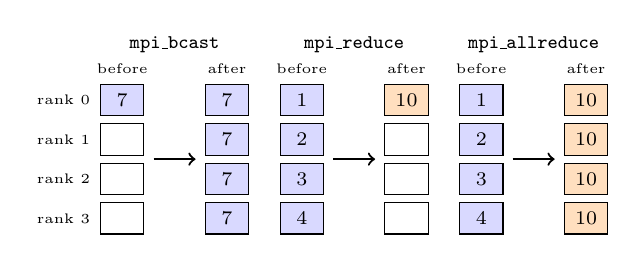
\begin{tikzpicture}[font=\scriptsize, x=0.95cm, y=0.5cm,
          box/.style={draw, minimum width=0.55cm, minimum height=0.4cm},
          full/.style={box, fill=blue!15},
          res/.style={box, fill=orange!25}]
        \foreach \name/\x in {mpi\_bcast/0, mpi\_reduce/2.4, mpi\_allreduce/4.8} {
          \node[font=\scriptsize\ttfamily] at (\x+0.7, 0.9) {\name};
          \node[font=\tiny] at (\x, 0.3) {before};
          \node[font=\tiny] at (\x+1.4, 0.3) {after};
          \draw[->, thick] (\x+0.42, -2.0) -- (\x+0.98, -2.0);
        }
        \foreach \r in {0,1,2,3} {
          \node[anchor=east, font=\tiny] at (-0.3, -\r-0.5) {rank \r};
        }
        % Broadcast
        \node[full] at (0, -0.5) {7};
        \foreach \r in {1,2,3} { \node[box] at (0, -\r-0.5) {}; }
        \foreach \r in {0,1,2,3} { \node[full] at (1.4, -\r-0.5) {7}; }
        % Reduce
        \foreach \r/\v in {0/1,1/2,2/3,3/4} { \node[full] at (2.4, -\r-0.5) {\v}; }
        \node[res] at (3.8, -0.5) {10};
        \foreach \r in {1,2,3} { \node[box] at (3.8, -\r-0.5) {}; }
        % Allreduce
        \foreach \r/\v in {0/1,1/2,2/3,3/4} { \node[full] at (4.8, -\r-0.5) {\v}; }
        \foreach \r in {0,1,2,3} { \node[res] at (6.2, -\r-0.5) {10}; }
      \end{tikzpicture}

      \vspace*{3mm}
      \footnotesize
      \raggedright
      \texttt{mpi\_bcast} copies the data of the root to every rank. \texttt{mpi\_reduce} combines the data of all the ranks, here with \texttt{MPI\_SUM}, into the root. \texttt{mpi\_allreduce} gives the result to every rank. Here, the root is rank 0.
    \end{column}
  \end{columns}
\end{frame}


\begin{frame}[fragile]
  \frametitle{Broadcast}
\begin{lstlisting}
call mpi_bcast(buffer, count, datatype, root, comm)
\end{lstlisting}
  \begin{columns}[T]
    \begin{column}{0.45\textwidth}
      \begin{itemize}
        \item On the root, \texttt{buffer} holds the data to send. On the other ranks, it receives the data.
        \item A common use: rank 0 reads the input, and broadcasts it to the others. With \texttt{mpirun}, only rank 0 can read the standard input.
      \end{itemize}

\begin{lstlisting}[language=bash]
$ echo 1000 | mpirun -np 4 ./bcast
 Rank           0 has n =        1000
 Rank           2 has n =        1000
 Rank           3 has n =        1000
 Rank           1 has n =        1000
\end{lstlisting}
    \end{column}

    \begin{column}{0.55\textwidth}
      \texttt{bcast.f90}:
\begin{lstlisting}
program bcast
  use mpi_f08
  implicit none
  integer :: rank, n

  call mpi_init()
  call mpi_comm_rank(MPI_COMM_WORLD, rank)

  if (rank == 0) read *, n    ! only rank 0 reads
  call mpi_bcast(n, 1, MPI_INTEGER, 0, MPI_COMM_WORLD)
  print *, 'Rank', rank, 'has n =', n

  call mpi_finalize()
end program bcast
\end{lstlisting}
    \end{column}
  \end{columns}
\end{frame}


\begin{frame}[fragile]
  \frametitle{Reduce and allreduce}
\begin{lstlisting}
call mpi_reduce(sendbuf, recvbuf, count, datatype, op, root, comm)
call mpi_allreduce(sendbuf, recvbuf, count, datatype, op, comm)
\end{lstlisting}
  \begin{columns}[T]
    \begin{column}{0.45\textwidth}
      \begin{itemize}
        \item The operation \texttt{op} combines the values of all the ranks: \texttt{MPI\_SUM}, \texttt{MPI\_PROD}, \texttt{MPI\_MAX}, \texttt{MPI\_MIN}, \ldots
        \item Arrays are combined element by element.
        \item \texttt{sendbuf} and \texttt{recvbuf} must be different variables. To combine into the same array, pass \texttt{MPI\_IN\_PLACE} as \texttt{sendbuf}.
        \item This is the MPI version of the OpenMP \texttt{reduction} clause.
      \end{itemize}
    \end{column}

    \begin{column}{0.55\textwidth}
      The total energy, on rank 0 only:
\begin{lstlisting}
call mpi_reduce(e, e_tot, 1, MPI_DOUBLE_PRECISION, &
                MPI_SUM, 0, MPI_COMM_WORLD)
\end{lstlisting}

      The largest speed, on every rank:
\begin{lstlisting}
call mpi_allreduce(v, v_max, 1, MPI_DOUBLE_PRECISION, &
                   MPI_MAX, MPI_COMM_WORLD)
\end{lstlisting}

      A histogram summed over all the ranks, in place:
\begin{lstlisting}
call mpi_allreduce(MPI_IN_PLACE, counts, n_bins, &
                   MPI_INTEGER, MPI_SUM, MPI_COMM_WORLD)
\end{lstlisting}
    \end{column}
  \end{columns}
\end{frame}


\begin{frame}[fragile]
  \frametitle{Dividing the work between the ranks}
  \begin{columns}[T]
    \begin{column}{0.5\textwidth}
      \begin{itemize}
        \item To share a loop over $n$ items between $p$ ranks, each rank computes its own block from its rank. No communication is needed.
        \item If $p$ does not divide $n$, the blocks differ in size by at most one:
      \end{itemize}
\begin{lstlisting}
i1 = rank * n / n_ranks + 1
i2 = (rank + 1) * n / n_ranks
do i = i1, i2
  ...
end do
\end{lstlisting}
      The integer division rounds down, so the blocks join without gaps or overlaps.
    \end{column}

    \begin{column}{0.5\textwidth}
      \centering
      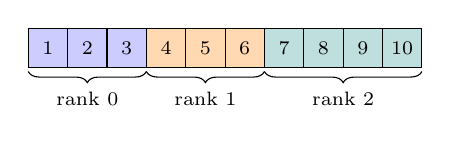
\begin{tikzpicture}[font=\scriptsize, x=0.5cm, y=0.5cm]
        \colorlet{r0}{blue!20}
        \colorlet{r1}{orange!30}
        \colorlet{r2}{teal!25}
        \foreach \i/\c in {1/r0,2/r0,3/r0,4/r1,5/r1,6/r1,7/r2,8/r2,9/r2,10/r2} {
          \draw[fill=\c] (\i-1,0) rectangle (\i,1);
          \node at (\i-0.5,0.5) {\i};
        }
        \draw[decorate, decoration={brace, mirror, amplitude=4pt}] (0,-0.1) -- (3,-0.1) node[midway, below=4pt] {rank 0};
        \draw[decorate, decoration={brace, mirror, amplitude=4pt}] (3,-0.1) -- (6,-0.1) node[midway, below=4pt] {rank 1};
        \draw[decorate, decoration={brace, mirror, amplitude=4pt}] (6,-0.1) -- (10,-0.1) node[midway, below=4pt] {rank 2};
      \end{tikzpicture}

      \vspace*{1mm}
      \footnotesize $n = 10$ items and $p = 3$ ranks.

      \vspace*{3mm}
      \raggedright
      \normalsize
      If the items take different amounts of work, a \emph{cyclic} division balances the load better, like \texttt{schedule(static, 1)} in OpenMP:
\begin{lstlisting}
do i = rank + 1, n, n_ranks
  ...
end do
\end{lstlisting}
    \end{column}
  \end{columns}
\end{frame}


\begin{frame}
  \frametitle{Example: the trapezoid rule}
  \begin{columns}[T]
    \begin{column}{0.5\textwidth}
      With $n$ trapezoids of width $h = (b - a) / n$,
      \[ \int_a^b f(x)\,\mathrm{d}x \approx h \left[ \frac{f(a) + f(b)}{2} + \sum_{i=1}^{n-1} f(a + ih) \right] \]
      \begin{itemize}
        \item Each rank sums $f$ over its own block of the inner points $i = 1, \ldots, n - 1$.
        \item \texttt{mpi\_reduce} adds the partial sums on rank~0.
        \item The end points must be added only once in total, so only rank 0 adds them.
        \item With $f(x) = 4 / (1 + x^2)$ on $[0, 1]$, the integral is $\pi$.
      \end{itemize}
    \end{column}

    \begin{column}{0.5\textwidth}
      \centering
      \footnotesize
      \begin{tabular}{rl}
        \textbf{Ranks} & \textbf{Result} ($n = 10^6$) \\
        \hline
        1 & 3.1415926535897927 \\
        2 & 3.1415926535895884 \\
        3 & 3.1415926535895680 \\
        4 & 3.1415926535895973 \\
        8 & 3.1415926535896328 \\
        \hline
        $\pi$ & 3.1415926535897932 \\
      \end{tabular}

      \vspace*{3mm}
      \raggedright
      \normalsize
      The last digits change with the number of ranks, because the partial sums are added in a different order. Floating-point addition is not associative.
    \end{column}
  \end{columns}
\end{frame}


\begin{frame}[fragile]
  \frametitle{The trapezoid rule with MPI}
  \begin{columns}[T]
    \begin{column}{0.5\textwidth}
\begin{lstlisting}[aboveskip=0pt, belowskip=0pt]
program trapezoid
  use mpi_f08
  use iso_fortran_env, only: dp => real64
  implicit none
  integer, parameter :: n = 1000000
  real(dp), parameter :: a = 0.0_dp, b = 1.0_dp
  integer :: rank, n_ranks, i, i1, i2
  real(dp) :: h, local, total

  call mpi_init()
  call mpi_comm_rank(MPI_COMM_WORLD, rank)
  call mpi_comm_size(MPI_COMM_WORLD, n_ranks)

  ! This rank's block of the inner points
  h = (b - a) / n
  i1 = rank * (n - 1) / n_ranks + 1
  i2 = (rank + 1) * (n - 1) / n_ranks

  local = 0.0_dp
  do i = i1, i2
    local = local + f(a + i * h)
  end do
\end{lstlisting}
    \end{column}

    \begin{column}{0.5\textwidth}
\begin{lstlisting}[aboveskip=0pt, belowskip=0pt]
  ! Add the end points only once in total
  if (rank == 0) then
    local = local + 0.5_dp * (f(a) + f(b))
  end if

  call mpi_reduce(local, total, 1, &
                  MPI_DOUBLE_PRECISION, MPI_SUM, &
                  0, MPI_COMM_WORLD)
  if (rank == 0) print *, 'Integral:', h * total

  call mpi_finalize()

contains

  pure real(dp) function f(x)
    real(dp), intent(in) :: x
    f = 4.0_dp / (1.0_dp + x**2)
  end function f

end program trapezoid
\end{lstlisting}
    \end{column}
  \end{columns}
\end{frame}


\begin{frame}[fragile]
  \frametitle{Timing}
  \begin{columns}[T]
    \begin{column}{0.5\textwidth}
      \begin{itemize}
        \item \texttt{mpi\_wtime()} returns the wall-clock time in seconds as a \texttt{real(real64)}, like \texttt{omp\_get\_wtime()}.
        \item Each rank has its own clock, so use only time differences.
        \item A parallel program is as fast as its slowest rank. Start the ranks together with \texttt{mpi\_barrier}, which waits until all the ranks reach it, and report the largest time.
        \item Amdahl's law (Lecture 10) holds for MPI too. The time spent in communication adds to the serial part.
      \end{itemize}
    \end{column}

    \begin{column}{0.5\textwidth}
\begin{lstlisting}
real(dp) :: t0, t, t_max

call mpi_barrier(MPI_COMM_WORLD)
t0 = mpi_wtime()

! ... the work ...

t = mpi_wtime() - t0
call mpi_reduce(t, t_max, 1, MPI_DOUBLE_PRECISION, &
                MPI_MAX, 0, MPI_COMM_WORLD)
if (rank == 0) print *, 'Time (s):', t_max
\end{lstlisting}

    \end{column}
  \end{columns}
\end{frame}


\section{Summary}

\begin{frame}
  \frametitle{Common pitfalls}
  \begin{columns}[T]
    \begin{column}{0.5\textwidth}
      \begin{itemize}
        \item \textbf{Work done once per rank.} Work that must be done once in total, such as output or the end points of a sum, needs an \texttt{if (rank == 0)}.
        \item \textbf{A wrong datatype or count.} The compiler cannot check them, and the result is wrong numbers, not an error.
        \item \textbf{Deadlock.} Two ranks that both wait for each other.
        \item \textbf{A collective called by only some ranks.} The others wait forever.
      \end{itemize}
    \end{column}

    \begin{column}{0.5\textwidth}
      \begin{itemize}
        \item \textbf{Output from many ranks.} The lines come in a random order. Print from rank 0.
        \item \textbf{Mixed MPI installations.} If \texttt{mpirun} is not from the same MPI as \texttt{mpifort}, every process says it is ``rank 0 of 1''. Check with \texttt{which mpifort mpirun}.
        \item \textbf{Testing with one rank only.} Compare the results with 1, 2, 3, and 4 ranks. An odd number of ranks finds bugs in the division of the work.
        \item \textbf{A hang.} Find the call in which each rank waits.
      \end{itemize}
    \end{column}
  \end{columns}
\end{frame}


\begin{frame}
  \frametitle{Summary}
  \begin{columns}[T]
    \begin{column}{0.55\textwidth}
      \centering
      \footnotesize
      \begin{tabular}{ll}
        \textbf{Routine} & \textbf{Meaning} \\
        \hline
        \texttt{mpi\_init}, \texttt{mpi\_finalize} & start and end MPI \\
        \texttt{mpi\_comm\_size}  & number of ranks \\
        \texttt{mpi\_comm\_rank}  & rank of this process \\
        \texttt{mpi\_send}, \texttt{mpi\_recv} & one message, blocking \\
        \texttt{mpi\_sendrecv}    & send and receive at once \\
        \texttt{mpi\_bcast}       & root's data to all \\
        \texttt{mpi\_reduce}      & combine data into the root \\
        \texttt{mpi\_allreduce}   & combine data into all \\
        \texttt{mpi\_barrier}     & wait for all the ranks \\
        \texttt{mpi\_wtime}       & wall-clock time \\
        \texttt{mpi\_abort}       & stop all the ranks \\
        \hline
      \end{tabular}

      \vspace*{2mm}
      \raggedright
      Compile with \texttt{mpifort}, and run with \texttt{mpirun -np N}.
    \end{column}

    \begin{column}{0.45\textwidth}
      \small
      \begin{itemize}
        \item The MPI standard: \\ \url{https://www.mpi-forum.org/docs/}
        \item Open MPI documentation: \\ \url{https://docs.open-mpi.org/}
        \item Books:
          \begin{itemize}
            \item W. Gropp, E. Lusk, A. Skjellum, \emph{Using MPI} (3rd ed., MIT Press, 2014),
            \item P.S. Pacheco, \emph{Parallel Programming with MPI} (Morgan Kaufmann, 1997).
          \end{itemize}
          Both use the older interfaces, but the routines are the same.
      \end{itemize}
    \end{column}
  \end{columns}
\end{frame}


\section{Exercises}

\begin{frame}{Exercise 1: a ring}
  \begin{block}{Tasks}
    \begin{enumerate}
      \item Arrange the ranks in a ring: rank $r$ sends to rank $(r + 1) \bmod p$, and receives from rank $(r - 1 + p) \bmod p$.
      \item Pass a token around the ring: rank 0 sends the value 0 to rank 1, every rank adds its rank to the value and passes it on, and rank 0 receives the final value from rank $p - 1$ and prints it. Check the result against $p(p - 1)/2$.
      \item Now let every rank send an array of $n$ numbers to its right neighbour, and receive one from its left neighbour, at the same time, with \texttt{mpi\_send} followed by \texttt{mpi\_recv}. Increase $n$ until the program deadlocks. Fix it with \texttt{mpi\_sendrecv}.
    \end{enumerate}
  \end{block}
\end{frame}


\begin{frame}{Exercise 2: Monte Carlo $\pi$}
  \begin{block}{Tasks}
    \begin{enumerate}
      \item Write a program that draws $N$ random points in the unit square, and counts how many fall inside the quarter circle $x^2 + y^2 < 1$. The fraction inside approaches $\pi / 4$.
      \item Share the $N$ points between the ranks, and combine the counts with \texttt{mpi\_reduce}. Rank 0 reads $N$ from the standard input, and broadcasts it.
      \item Give every rank a different seed with \texttt{random\_seed(put=...)}. What goes wrong if all the ranks use the same seed?
      \item Time the program with \texttt{mpi\_wtime} for $N = 10^8$ and 1, 2, 4, and 8 ranks, and compute the speedups.
    \end{enumerate}
  \end{block}
\end{frame}


\begin{frame}{Exercise 3: the trapezoid rule}
  \begin{block}{Tasks}
    \begin{enumerate}
      \item Change \texttt{trapezoid.f90} so that rank 0 reads $a$, $b$, and $n$ from the standard input, and broadcasts them to the other ranks.
      \item Check that the result does not depend on the number of ranks, for $n$ divisible and not divisible by the number of ranks.
      \item Time the program with \texttt{mpi\_wtime} for $n = 10^8$ with 1, 2, 4, and 8 ranks, and compare the speedups with Amdahl's law.
      \item With $n = 10^9$ and four ranks, the program gives a wrong result. Why? Fix it. (Hint: \texttt{huge(1)}.)
    \end{enumerate}
  \end{block}
\end{frame}

\end{document}
